\documentclass[a4paper,12pt]{article}
\usepackage[a4paper, top=2cm,bottom=2cm,right=2cm,left=2cm]{geometry}

\usepackage{bm,xcolor,mathdots,latexsym,amsfonts,amsthm,amsmath,
					mathrsfs,graphicx,cancel,tikz-cd,hyperref,booktabs,caption,amssymb,amssymb,wasysym}
\hypersetup{colorlinks=true,linkcolor=blue}
\usepackage[italian]{babel}
\usepackage[T1]{fontenc}
\usepackage[utf8]{inputenc}
\newcommand{\s}[1]{\left\{ #1 \right\}}
\newcommand{\sbarra}{\backslash} %% \ 
\newcommand{\ds}{\displaystyle} 
\newcommand{\alla}{^}  
\newcommand{\implica}{\Rightarrow}
\newcommand{\iimplica}{\Leftarrow}
\newcommand{\ses}{\Leftrightarrow} %se e solo se
\newcommand{\tc}{\quad \text{ t. c .} \quad } % tale che 
\newcommand{\spazio}{\vspace{0.5 cm}}
\newcommand{\bbianco}{\textcolor{white}{,}}
\newcommand{\bianco}{\textcolor{white}{,} \\}% per andare a capo dopo 																					definizioni teoremi ...


% campi 
\newcommand{\N}{\mathbb{N}} 
\newcommand{\R}{\mathbb{R}}
\newcommand{\Q}{\mathbb{Q}}
\newcommand{\Z}{\mathbb{Z}}
\newcommand{\K}{\mathbb{K}} 
\newcommand{\C}{\mathbb{C}}
\newcommand{\F}{\mathbb{F}}
\newcommand{\p}{\mathbb{P}}

%GEOMETRIA
\newcommand{\B}{\mathfrak{B}} %Base B
\newcommand{\D}{\mathfrak{D}}%Base D
\newcommand{\RR}{\mathfrak{R}}%Base R 
\newcommand{\Can}{\mathfrak{C}}%Base canonica
\newcommand{\Rif}{\mathfrak{R}}%Riferimento affine
\newcommand{\AB}{M_\D ^\B }% matrice applicazione rispetto alla base B e D 
\newcommand{\vett}{\overrightarrow}
\newcommand{\sd}{\sim_{SD}}%relazione sx dx
\newcommand{\nvett}{v_1, \, \dots , \, v_n} % v1 ... vn
\newcommand{\ncomb}{a_1 v_1 + \dots + a_n v_n} %a1 v1 + ... +an vn
\newcommand{\nrif}{P_1, \cdots , P_n} 
\newcommand{\bidu}{\left( V^\star \right)^\star}

\newcommand{\udis}{\amalg}
\newcommand{\ric}{\mathfrak{U}}
\newcommand{\inclu}{\hookrightarrow }
%ALGEBRA

\newcommand{\semidir}{\rtimes}%semidiretto
\newcommand{\W}{\Omega}
\newcommand{\norma}{\vert \vert }
\newcommand{\bignormal}{\left\vert \left\vert}
\newcommand{\bignormar}{\right\vert \right\vert}
\newcommand{\normale}{\triangleleft}
\newcommand{\nnorma}{\vert \vert \, \cdot \, \vert \vert}
\newcommand{\dt}{\, \mathrm{d}t}
\newcommand{\dz}{\, \mathrm{d}z}
\newcommand{\dx}{\, \mathrm{d}x}
\newcommand{\dy}{\, \mathrm{d}y}
\newcommand{\amma}{\gamma}
\newcommand{\inv}[1]{#1^{-1}}
\newcommand{\az}{\centerdot}
\newcommand{\ammasol}[1]{\tilde{\gamma}_{\tilde{#1}}}
\newcommand{\pror}[1]{\mathbb{P}^#1 (\R)}
\newcommand{\proc}[1]{\mathbb{P}^#1(\C)}
\newcommand{\sol}[2]{\widetilde{#1}_{\widetilde{#2}}}
\newcommand{\bsol}[3]{\left(\widetilde{#1}\right)_{\widetilde{#2}_{#3}}}
\newcommand{\norm}[1]{\left\vert\left\vert #1 \right\vert \right\vert}
\newcommand{\abs}[1]{\left\vert #1 \right\vert }
\newcommand{\ris}[2]{#1_{\vert #2}}
\newcommand{\vp}{\varphi}
\newcommand{\vt}{\vartheta}
\newcommand{\wt}[1]{\widetilde{#1}}
\newcommand{\pr}[2]{\frac{\partial \, #1}{\partial\, #2}}%derivata parziale
%per creare teoremi, dimostrazioni ... 
\theoremstyle{plain}
\newtheorem{thm}{Teorema}[section] 
\newtheorem{ese}[thm]{Esempio} 
\newtheorem{ex}[thm]{Esercizio} 
\newtheorem{fatti}[thm]{Fatti}
\newtheorem{fatto}[thm]{Fatto}

\newtheorem{cor}[thm]{Corollario} 
\newtheorem{lem}[thm]{Lemma} 
\newtheorem{al}[thm]{Algoritmo}
\newtheorem{prop}[thm]{Proposizione} 
\theoremstyle{definition} 
\newtheorem{defn}{Definizione}[section] 
\newcommand{\intt}[2]{int_{#1}^{#2}}
\theoremstyle{remark} 
\newtheorem{oss}{Osservazione} 
\newcommand{\di }{\, \mathrm{d}}
\newcommand{\tonde}[1]{\left( #1 \right)}
\newcommand{\quadre}[1]{\left[ #1 \right]}
\newcommand{\w}{\omega}

% diagrammi commutativi tikzcd
% per leggere la documentazione texdoc

\begin{document}
\textbf{Lezione del 27 aprile}
\begin{thm}[dei residui]\bianco
Sia $D\subseteq \C$ un aperto, sia $f:\, D \setminus S $ olomorfa con $S$ chiuso e discreto in $D$.\\
Sia $R\subseteq D$ compatto con bordo $C^1$ a tratti, dunque  $R\cap S=\{ z_1, \dots, z_k\}$ \`e finito,   $\partial R \cap S =\emptyset$.\\
Allora 
$$\int_{\partial R} f(z) \dz =2\pi  i\sum_{i=1}^k Res(f,z_i)$$
\proof Lo dimostriamo solamente nel caso in cui $D$ \`e omeomorfa ad un disco.\\
Consideriamo i cammini come in figura
\begin{figure}[!h]
\centering
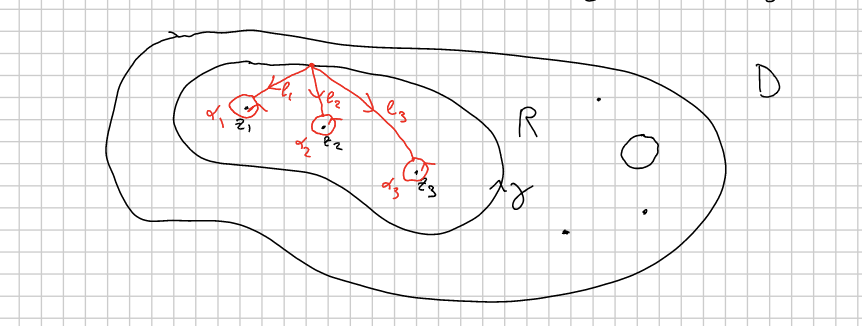
\includegraphics[scale=0.5]{Figure/04_27}
\end{figure}
dove $\alpha_i$ \`e una piccola circonferenza intorno a $z_i$ percorsa in senso antiorario.\\
Consideriamo il cammino
$$ \beta  =\gamma\star l_k \star \overline{\alpha_k}\star \overline{l_k} \star l_{k-1}\star \overline{\alpha_{k-1}} \star \overline{l_{k_1}} \star \dots \star l_1 \star \overline{\alpha_1}\star \overline{l_1}$$
tale cammino \`e omotopicamente banale in $R \setminus S $ poich\`e borda un disco ed essendo $f$ olomorfa $\w=f\dz  $\`e chiusa su $R\setminus S$  si ha 
$$ 0=\int_\beta \w = \int_\gamma \w +\sum_{i=1}^k \tonde{ \cancel{\int_{\overline{l_i}} \w } + \int_{\overline{\alpha_i}} \w +\cancel{\int_{l_i} \w } }$$ 
da cui otteniamo 
$$ \int_\gamma \w = -\sum_{i=1}^k \int_{\overline{\alpha_i}}\w =\sum_{i=1}^k \int_{\alpha_i} \w = 2\pi i \sum_{i=1}^k Res(f,z_i)$$
La dimostrazione nel caso in cui $R$ non sia un omemorfa ad un disco \`e simile ma non viene dimostrato
\end{thm}
\subsection{Calcolo di residui}
Se $z_0$ \`e un polo semplice di $f$, allora
$$ f(z) = \frac{a_{-1}}{z-z_0}+\sum_{n\geq 0} a_n (z-z_0)^n$$
dunque $$(z-z-0)f(z) = a_{-1} \sum_{n \geq 0 } a_n(z-z_0)^{n+1} $$ da cui 
$$Res(f,z_0) = a_{-1}=\lim_{z\to z_0} (z-z_0) f(z)$$
Nel caso $f=\frac{P}{Q}$ con $P,Q$ olomorfe $P(z_0)\neq 0 $ e $z_0$ zero semplice di $Q$ otteniamo 
$$ Res(f,z_0) = \lim_{z\to z_0} \frac{(z-z_0)P(z)}{Q(z)} =\frac{P(z_0)}{Q'(z_0)}$$
\begin{ese}Calcolo dei residui di $f(z) = \frac{e^{iz}}{z^2 +1}$\\
$f(z)$ ha singolarit\`a in $z_0=i$ e $z_1=-1$ inoltre tali singolarit\`a sono poli semplici, essendo zero semplici di $z^2+1$.\\
Per quanto mostrato in precedenza otteniamo 
$$ Res(f,z_0) = \left. \frac{e^{iz}}{2z}\right]_{z=i} = \frac{e^{i^2}}{2i} =\frac{-i}{2e}$$
In modo analogo otteniamo 
$$ Res(f,z_1) = \frac{e^{i\cdot (-i)}}{2(-i)} = \frac{ei}{2}$$
\end{ese}
Mostriamo ora una strategia nel caso i poli non siano semplici.\\
Se $f$ ha un polo di ordine $k$ in $z_0$ si pone $g(z)=(z-z_0)^k f(z)$ che si estende ad una funzione olomorfa in $z_0$ (la denotiamo sempre con $g$).\\
Ora se 
$$f(z) = \sum_{n \in \Z} a_n z^n $$ 
si ha che $a_{-1}$ \`e il coefficiente di $(z-z_0)^{k-1} $ nello sviluppo di $g$.\\
Essendo $g$ olomorfa in $z_0$ si ha 
$$Res(f,z_0) = a_{-1}=\frac{g^{(k-1)}(z_0)}{(k-1)!}$$
\begin{ese}$f(z)=\frac{e^{iz}}{z(z^2+1)^2}$ ha un polo semplice in $0$ e due poli doppi in $\pm i$.\\
Per calcolare il residuo in $i$ consideriamo
$$g(z) = f(z) (z-i)^2=\cancel{(z-i)^2}\frac{e^{iz}}{z(z+i)^2\cancel{(z-i)^2}} =\frac{e^{iz}}{z(z+i)^2}$$
dunque 
$$g'(z) = \frac{ie^{iz}z(z+1)^2 - e^{iz} \tonde{(z+1)^2 +2z(z+i)}}{z^2(z+i)^4} $$
ovvero
$$g'(i) = -\frac{3}{4e} = \frac{g'(i)}{1!} =Res(f,i)$$

\newpage
\subsection{Applicazione del teorema dei residui}
\begin{ese}Calcolare 
$$ \int_{-\infty}^{+\infty} \frac{\cos x }{x^2+1}$$
L'integrale richiesto \`e equivalente al calcolo di 
$$ \lim_{R \to + \infty} \int_{-R}^R \frac{\cos  x}{x^2 + 1 }$$
Notiamo ora che se $x\in \R$ allora $\frac{\cos x}{x^2 +1} =Re \tonde{\frac{e^{iz}}{z^2 +1 }}$.\\
La funzione $f(z) =\frac{e^{iz}}{z^2 +1 }$ ha poli semplici in $\pm i$.\\
Sia $$\Omega_R = \{ z\in \C \, : \, \abs{z} \leq R \text{ e } Im(z) \geq 0 \}$$
Una parametrizzazione positiva di $\Omega_R$ \`e $\alpha_R \star \beta_R$ come in figura 
\begin{figure}[!h]
\centering
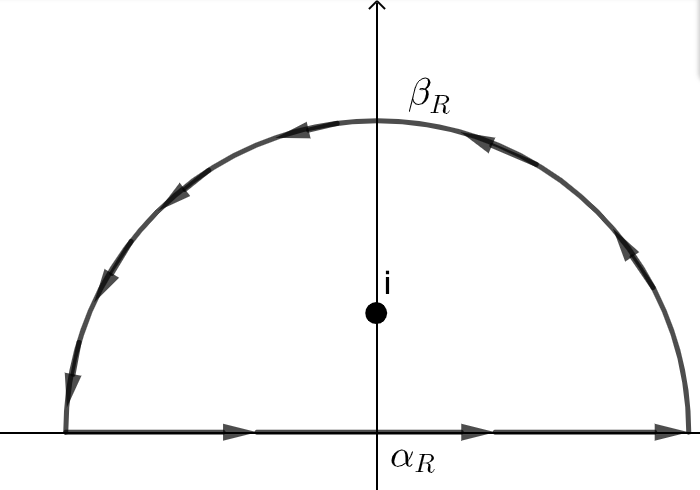
\includegraphics[scale=.5]{Figure/04_27_1}
\end{figure}
Per il teorema dei residui si ha 
$$\int_{\alpha_R} f(z) \dz +\int_{\beta_R} f(z) \dz = 2\pi i Res(f,i) = 2\pi i \tonde{\frac{-i}{2e} }=\frac{\pi}{2}$$
Essendo 
$$\alpha_R:\, [-R,R]\to \C \quad \alpha_R(t) = t$$
$$\beta_R:\, [0, \pi]\to \C \quad \beta_R(t) = R e^{it}$$
si ha 
$$ \int_{\alpha_R} f(z) \dz = \int_{-R}^R f(t) \alpha'(t)= \int_{-R}^R f(t) \dt = \int_{-R}^R \frac{\cos t + i\sin t}{t^2 +1} \dt $$
la cui parte reale \`e l'integrale richiesto (come limite).\\
Per concludere osserviamo che $\int_{\beta_R} f(z) \dz = 0$.\\
Ora $\beta_R(t)=R^{e^it}= R(\cos t + i \sin t)$ per cui 
$$e^{i\beta_R(t)} = e^{iR(\cos t+ i \sin t) } = e^{iR \cos t } e^{-R \sin t }\quad \implica \quad \abs{f(\beta_R(t))}=e^{-R\sin t }$$
da cui 
$$ \abs{f(\beta_R(t) \beta_R'(t) } =\abs{\frac{e^{i\beta_R(t)}}{\beta_R(t)^2 + 1} i R e^{it}}=\frac{e^{-R\sin t} }{R^2 e^{2it}+1} \leq \frac{R}{R^2 +1}$$ 
per cui 
$$ \abs{\int_{\beta_R} f(z) \dz } \leq \int_0^\pi \frac{R}{R^2 +1} \dt  = \frac{R \pi }{R^2 +1} \to 0 \text{ per } R \to +\infty$$
Dunque abbiamo 
$$ \int_{-\infty}^{\infty} \frac{\cos x }{x^2 + 1}\dx = \frac{\pi}{e}$$
\end{ese}
\begin{oss}Per ``complessificare" la funzione si sarebbe potuto prendere $\frac{\cos z }{z^2 +1}$.\\
Il problema \`e che $\abs{\frac{\cos z }{z^2 +1}}$ non \`e stimabile facilmente lungo $\beta_R(t)$, inoltre $\cos (i t) = \cosh t $ che non \`e limitato
\end{oss}
\begin{oss}In modo analogo (sempre integrando lungo $\partial \W_R$ con $\W_R$ come sopra) si calcola
$$ \int_{-\infty}^\infty \frac{P(x)}{Q(x)}\text{ dove } P, Q \text{ polinomi, } Q(x)  \neq  0 \text{ e } \deg Q > \deg P+2 $$
\end{oss}
\spazio
\begin{ese}Calcolare
$$ \int_{-\infty}^\infty \frac{1}{1+x^4}\dx $$ 
Se consideriamo la funzione complessa $f(z) = \frac{1}{1+z^4}$ essa ha $4$ poli, la  regione $\Omega_R$ (come sopra)  contiene solamente i poli $z_0=e^{i \frac{\pi}{4}}$ e $z_1=e^{i\frac{3}{4}\pi }$ che sono semplici.\\
Ragionando come sopra otteniamo
$$ \int_{\partial\W_R} f(z) \dz = 2\pi i ( Res(f,z_0) + Res(f,z_1)) =2\pi i \tonde{-\frac{z_0}{4}- \frac{z_1}{4}} =\frac{\sqrt{2}}{2}\pi$$
come prima otteniamo che $\int_{\beta_R} f(z)\dz \to 0 $ per $R \to +\infty$ da cui 
$$ \int_{-\infty}^\infty\frac{1}{1+x^2} \dx = \frac{\sqrt{2}}{2}\pi $$
\end{ese}








\end{ese}
\end{document}